\documentclass[aspectratio=169]{beamer}

\usetheme{Rochester}
\usecolortheme{default}
\usefonttheme{structurebold}

\usepackage[skip=6pt]{parskip}
\usepackage{graphicx}
\graphicspath{{static}}

\setbeamertemplate{navigation symbols}{}

\title{Package Assignment and Routing System (PARS)}
\author{%
    Lakshay Bansal,
    Mathew Robotham,
    Young Shin
}
\institute{University at Albany, SUNY}
\date{\today}

\begin{document}

\begin{frame}[plain]
    \titlepage
\end{frame}

\begin{frame}{Introduction}
    \begin{itemize}
        \item Suppose you're a warehouse operator serving a city.
        \item Your job is to distribute goods from the warehouse using delivery trucks to transport them to their final destination in an efficient manner.
        \item However, a single truck can carry far more than just one delivery at a time.
        \item As such, we must design efficient routes for these trucks.
    \end{itemize}

    \begin{center}
        \raisebox{0\height}{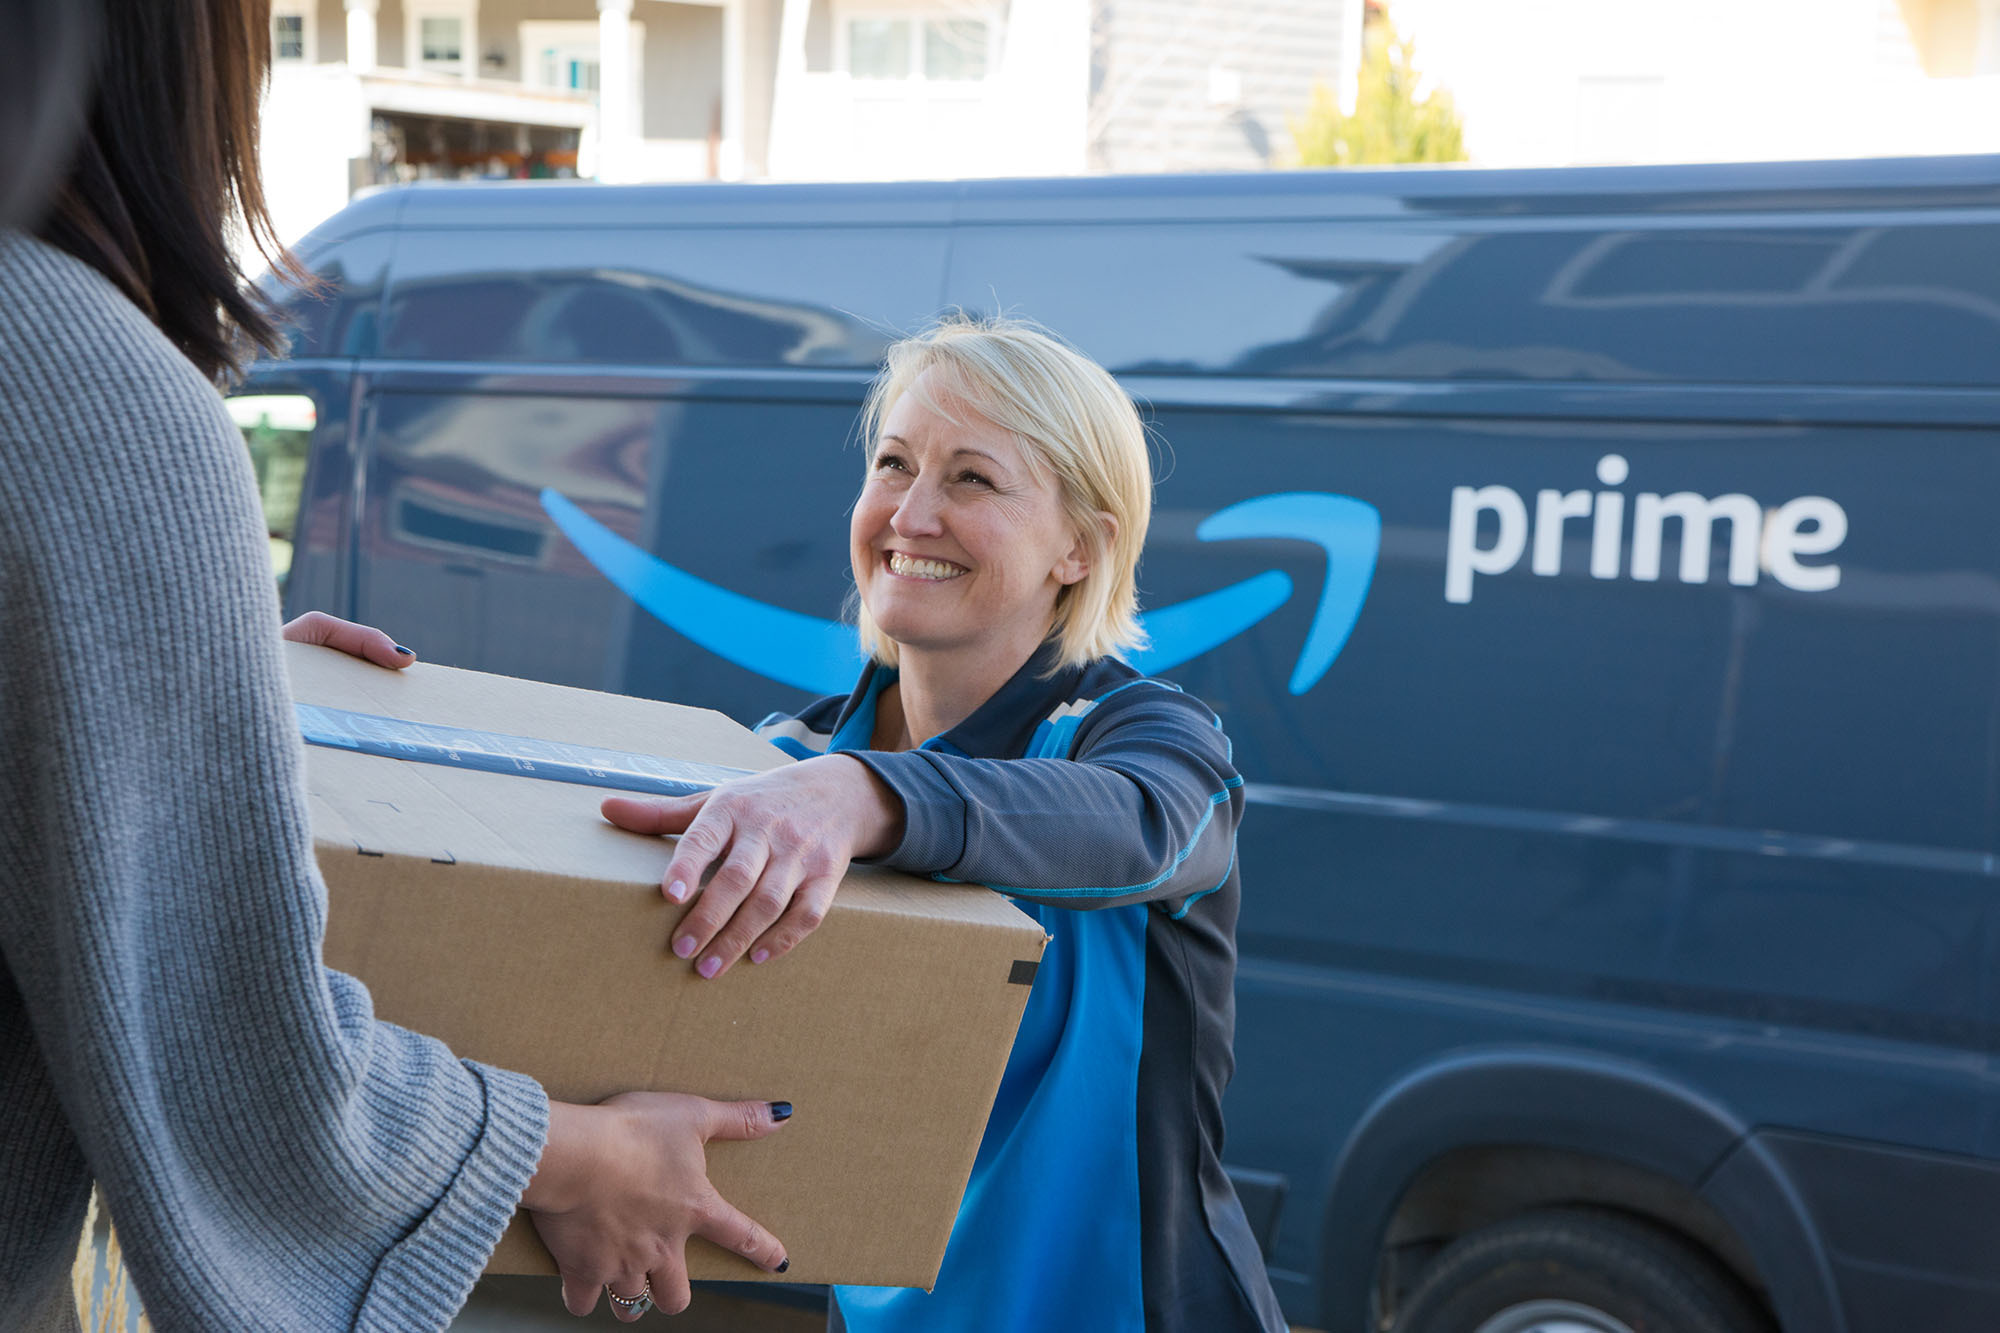
\includegraphics[width=.35\linewidth]{dsp.jpg}}\quad
        \raisebox{0\height}{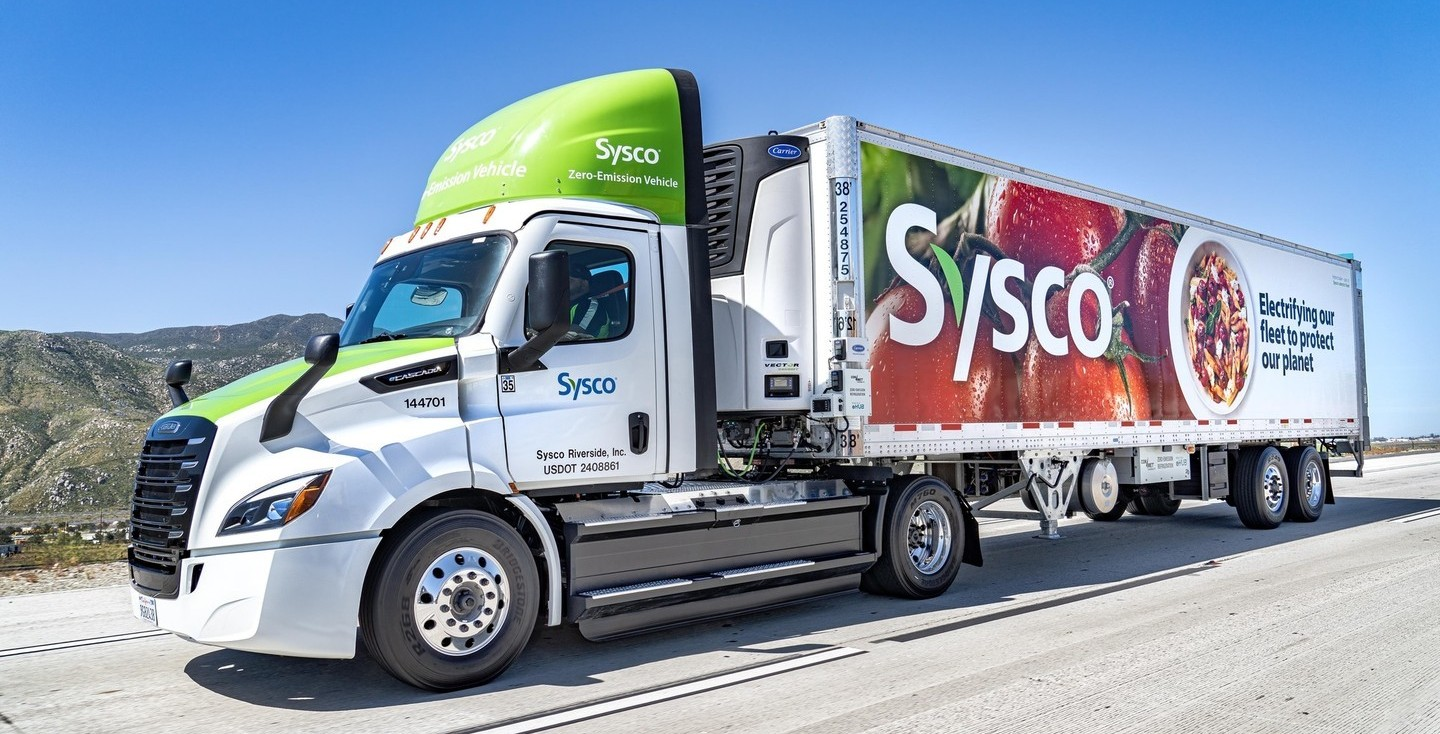
\includegraphics[width=.48\linewidth]{sysco.jpg}}
    \end{center}
\end{frame}

\begin{frame}{Motivation}
    For our project we'll be using the analogy of delivering packages to homes.
    \begin{itemize}
        \item Consider, school bus routing, human and robotic warehouse pickers/stockers, waste collection, snow plowing, coordination of emergency services, etc.
        \item Finding an optimal solution is computationally expensive. Must resort to heuristics to find a reasonable solution in a reasonable amount of time.
        \item AI revolves around this idea of making good enough decisions in a reasonable amount of time.
    \end{itemize}

    \begin{center}
        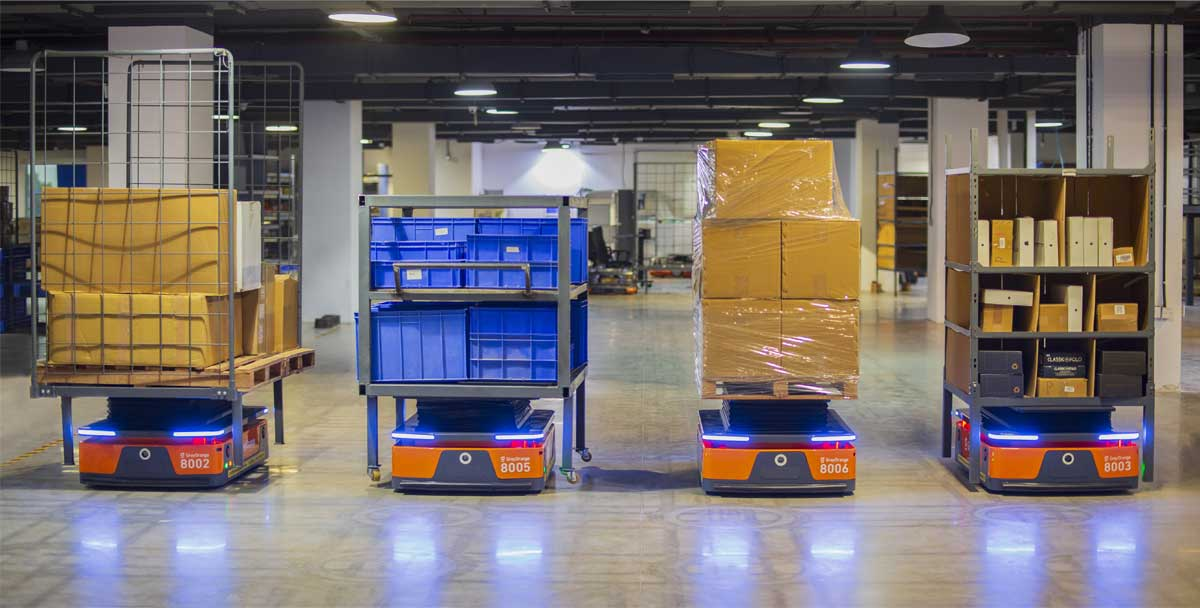
\includegraphics[width=.4\linewidth]{warehouse.jpeg}\quad
        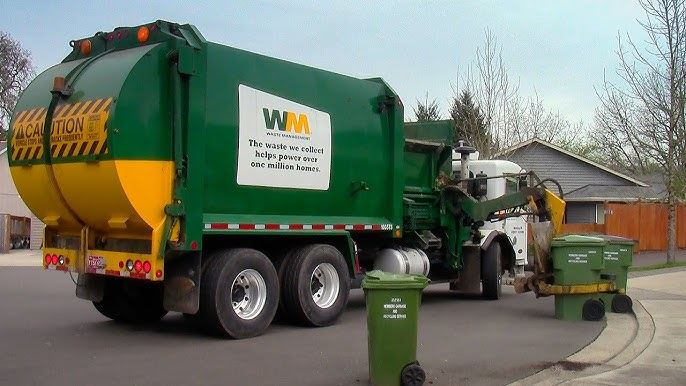
\includegraphics[width=.38\linewidth]{garbage-truck.jpg}
    \end{center}
\end{frame}

\begin{frame}{Foundational problem}
    \textbf{Traveling salesman problem (TSP)} --- ``Given some origin city, what's the shortest possible route that visits each city exactly once and returns to the origin city?''
    \begin{itemize}
        \item Modeling this as a graph theory problem, we can assume a complete graph $K_n$ where nodes are cities and edge weights are pre-calculated distances.
    \end{itemize}
    \begin{minipage}{.5\linewidth}
        \centering\small
        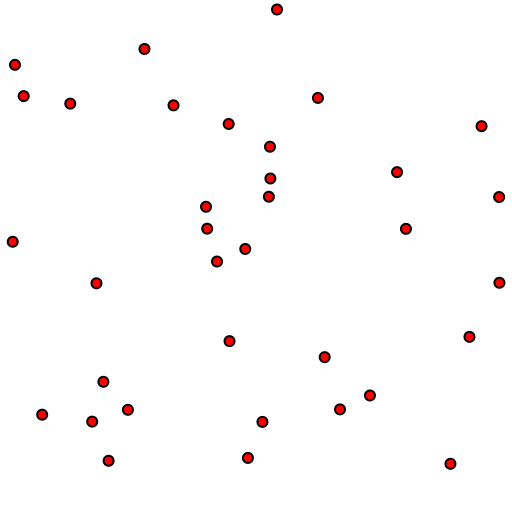
\includegraphics[width=.55\linewidth]{Illustration_of_an_unsolved_travelling_salesman_problem.png}\par
        Unsolved
    \end{minipage}%
    \begin{minipage}{.5\linewidth}
        \centering\small
        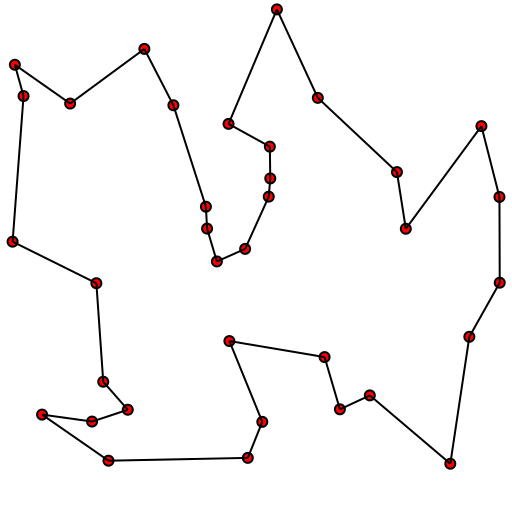
\includegraphics[width=.55\linewidth]{GLPK_solution_of_a_travelling_salesman_problem.png}\par
        Solved
    \end{minipage}
\end{frame}

\begin{frame}{Vehicle routing problem}
    \textbf{Vehicle routing problem (VRP)} --- Generalization of the traveling salesman problem which asks ``what is the optimal set of routes for a fleet of vehicles to traverse in order to deliver to a given set of customers?''
    \begin{itemize}
        \item Typically, goal is to minimize the total distance traveled by all vehicles, however, many more metrics might be considered.
        \item Can include any number of constraints that must be satisfied---a vehicle can only carry so much weight, a driver can only work for so long.
        \item Can be thought of as attempting to solve multiple traveling salesman problems or a multi-agent search problem.
    \end{itemize}
    VRPs usually still assume a complete graph where actual road routing is abstracted away. However, we will perform our VRP over graph which models a real-world road network.
\end{frame}

\begin{frame}{VRP overview}
    \begin{center}
        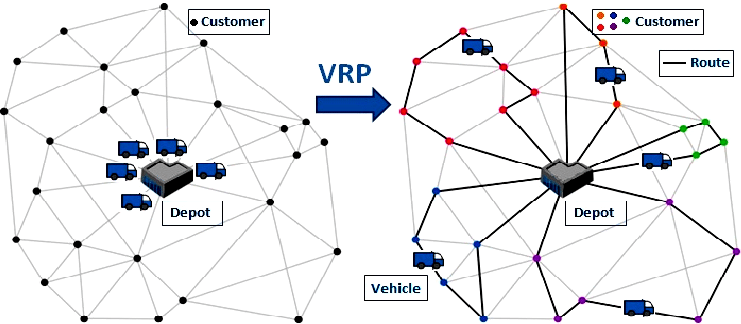
\includegraphics[width=.9\linewidth]{Classical-Vehicle-Routing-Problem.png}
    \end{center}
    {\footnotesize Gupta, Ashima \& Saini, Sanjay. (2017). An Enhanced Ant Colony Optimization Algorithm for Vehicle Routing Problem with Time Windows. 267-274. 10.1109/ICoAC.2017.8441175.}
\end{frame}

% \begin{frame}{Introduction}
%     \begin{center}
%         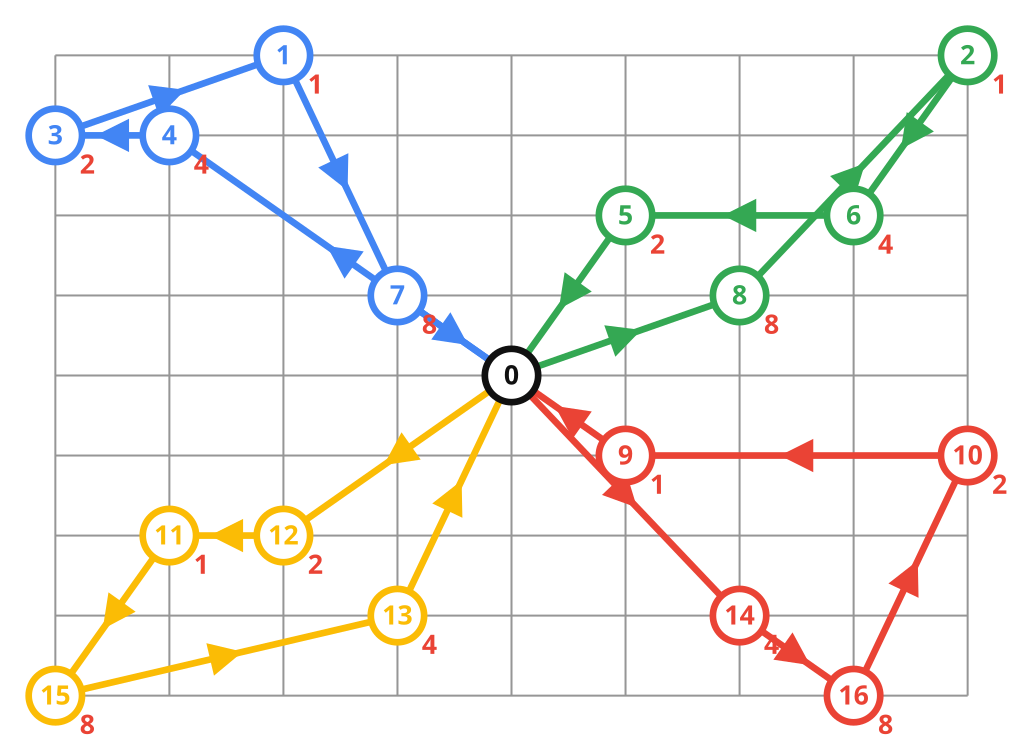
\includegraphics[width=.6\linewidth]{cvrp_solution.png}
%     \end{center}
%     {\footnotesize\url{https://developers.google.com/optimization/routing/cvrp}}
% \end{frame}

\begin{frame}{Formal definition}
    Let $G=(V,E)$ be a connected, weighted graph where
    \begin{itemize}
        {\parskip=0pt
        \item vertices represent intersecting roads and/or customers,
        \item vertices also possess latitude/longitude information $(x,y)$,
        \item all trucks start and end at a central warehouse described by a node $w\in V$,
        \item $C\subseteq V\setminus\{w\}$ is the set of destinations (customers) the trucks must visit,
        \item edges represent the existence of a road connecting two vertices where edge weights describe the distance between the two nodes.}
    \end{itemize}
    Let $T$ be a set of trucks each with fixed capacity $k$ where the total customers a single truck visits cannot exceed $k$.

    We define function $\text{PARS}(G,w,C,T,k)$ which outputs a mapping $T\to\{(w,\dots,w)\subseteq V,\dots\}$ which describes the route of each truck starting at $w$ and ending at $w$. The goal of this function is to minimize the total distance traveled, the sum of edge weights, across all trucks.
\end{frame}

% \begin{frame}{Formal definition}
%     Given some number of parcels, some number of delivery trucks, and an undirected weighted graph where
%     \begin{itemize}
%         {\parskip=0pt
%         \item nodes indicate intersections or destinations,
%         \item edge weights indicate the travel distance between two nodes,
%         \item each parcel has a single destination,
%         \item each truck can only carry a certain number of parcels, and that
%         \item every truck starts and ends at some node,}
%     \end{itemize}
%     devise a route for each truck that minimizes the total distance traveled by all trucks.
% \end{frame}

\begin{frame}{Our proposal}
    \begin{enumerate}
        \item Solve a single TSP (this is equivalent to having a single truck with an infinite capacity) using nearest-neighbor heuristic and A* search.
        \item Effectively, partition this route among vehicles
        \item Use $k$-means clustering to partition nearby customers and solving a TSP for each cluster.
        \item Use modern AI techniques like reinforcement learning to attempt to find more optimal solutions over our classical approaches.
    \end{enumerate}
    Our primary goal is to reduce the distance traveled by all trucks in total. We will record this metric, then compare and contrast different techniques and iterations of our solution.
\end{frame}

\begin{frame}{Main reference}

\end{frame}

\begin{frame}{Progress so far}
    \begin{center}
        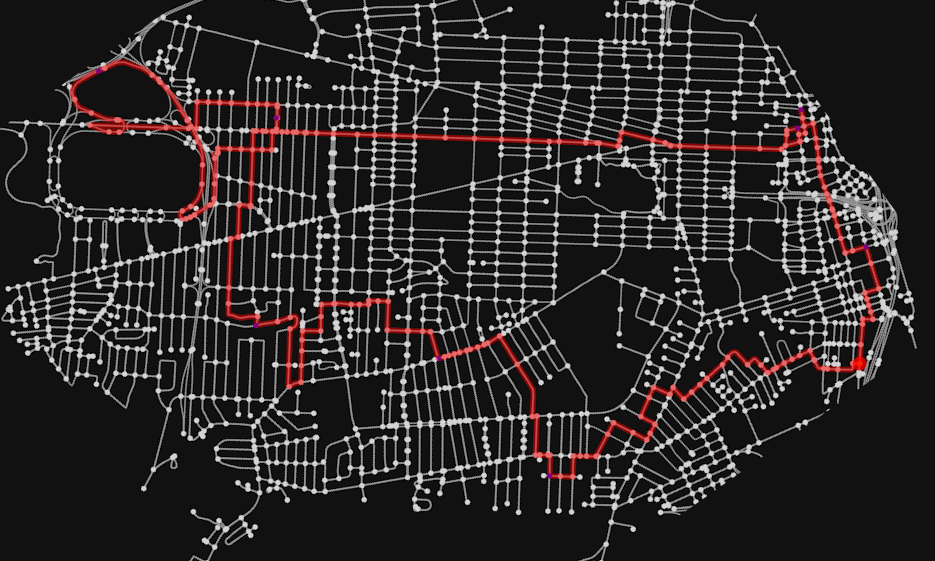
\includegraphics[width=.70\linewidth]{tsp_nn_solution.png}

        An 8-customer TSP solved using nearest neighbor heuristic (for picking the next node to visit) and A* search (for navigation between nodes) in Albany.
    \end{center}
\end{frame}

\begin{frame}[plain]
    \centering\LARGE\textbf{Thank you!}
\end{frame}

\end{document}
